\section{Introdu\c{c}\~ao}

\label{sec:introduction}
% For two-column wide figures use
\begin{figure}
% Use the relevant command to insert your figure file.
% For example, with the graphicx package use
\centering
  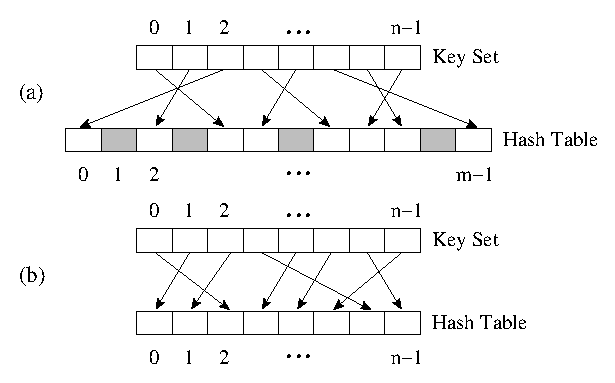
\includegraphics[width=0.45\textwidth, height=0.3\textheight]{figs/minimalperfecthash-ph-mph.ps}
% figure caption is below the figure
\caption{(a) Perfect hash function\quad  (b) Minimal perfect hash function}
\label{fig:minimalperfecthash-ph-mph}
\end{figure}

A efici\^encia dos algoritmos ser\'a medida atrav\'es das seguintes m\'etricas:
\begin{enumerate}
\item Quantidade de tempo gasto para encontrar uma fun\c{c}\~ao hash perfeita m\'{\i}nima $h$.
\item Quantidade de tempo necess\'ario para avaliar ou computar $h$.
\item Quantidade de mem\'oria exigida para armazenar a descri\c{c}\~ao da fun\c{c}\~ao $h$.
\item Quantidade de mem\'oria exigida para encontrar $h$.  
\item Escalabilidade dos algoritmos a medida que o conjunto de chaves cresce. 
\end{enumerate}

